\documentclass{article}
\usepackage[margin=1in]{geometry}
\usepackage{amsmath, amssymb, amsthm}
\usepackage{enumitem}

%Multiple Columns
\usepackage{multicol}

%Drawing Graphs
\usepackage{tikz}

%Cases Environment
\newlist{Cases}{enumerate}{3}
\setlist[Cases]{leftmargin = .25in, label = {Case \arabic*.}, topsep = 0.01in, itemsep = 0.04in, itemindent = .5in, parsep = 0in}

%Formatting and Spacing
\setitemize[1]{noitemsep, parsep = 5pt, topsep = 5pt}
\setenumerate[1]{label = (\alph*), parsep = 1pt, topsep = 5pt}
\setlength\parindent{0pt}
\linespread{1.15}

%Custom Title Fields
\newcommand{\lectTitle}{Lecture 5 Notes}
\newcommand{\lectTime}{January 26, 2022}
\newcommand{\lectClass}{Honors Discrete Mathematics}
\newcommand{\lectClassInstructor}{Professor Gerandy Brito}
\newcommand{\lectSection}{Spring 2022}
\newcommand{\lectAuthorName}{Sarthak Mohanty}

%Fancy Footnotes
\newcommand{\fancyfootnotetext}[2]{
  \fancypagestyle{dingens}{\fancyfoot[LO]{\parbox{6cm}{\footnotemark[#1]\footnotesize #2}}}\thispagestyle{dingens}
 }

%Headers and Footers
\usepackage{fancyhdr}
\usepackage{extramarks}
\pagestyle{fancy}
\lhead{\lectTime}
\chead{\lectClass \ (\lectClassInstructor)}
\rhead{\lectTitle}
\cfoot{\thepage}
\renewcommand\headrulewidth{0.4pt}
\renewcommand\footrulewidth{0.4pt}

\title{
    \vspace{2in}
    \textbf{\lectClass:\\ \lectTitle}\\
    \vspace{0.1in}\large{\textit{\lectClassInstructor\ \lectSection}}
    \vspace{3in}
    \author{\textbf{\lectAuthorName}}
    \date{}
}

\begin{document}

\maketitle
\pagebreak

\section*{Set Theory}
    \textbf{Definition:} A \textit{set} is an unordered collection of objects. They are the ``building blocks" of modern mathematics. Many of the symbols we have used so far are sets: some examples are $\mathbb{Q}$ and $\mathbb{R}$.

\subsection*{Notation}
    \begin{itemize}
        \item We denote sets using braces. Sets can be finite or infinite: For example, we define the set of natural numbers as $\{1, 2, 3, \dots\}$ and the set of natural numbers less than $100$ as $\{1, 2, 3, \dots, 99\}$.
        \item We denote an element $n$ residing in a set $S$ by $n \in S$. If $n$ is not in the set $S$, we say $n \notin S$.
        \item Sets can also be defined by predicates. The set of all elements $x$ in domain $D$ satisfying $P(x)$ is denoted with $\{x \in D : P(x)\}$ and is known as \textit{set-builder notation}.
        \item $A$ is a \textit{subset} of $B$ iff every element of $A$ is also an element in $B$; in other words, if $(\forall a \in D)(a \in A \Rightarrow a \in B)$. We denote this by $A \subseteq B$.
        \item Two sets are \textit{equal} iff they both contain exactly the same members; in other words, $X = (Y \iff X \subseteq Y) \land (Y \subseteq X)$.
        \item The \textit{cardinality}, or size, of a finite set $A$, is denoted with $|A|$.
    \end{itemize}
    
\subsection*{Operations}
    There are four main set operations.
    \begin{itemize}
        \item The intersection of two or more sets is the set $\{a \in D : a \in A \land a \in B\}$ and is denoted using $\cap$.
        \item The union of sets is the set $\{a \in D : a \in A \land a \in B\}$ and is denoted using $\cup$.
        \item The symmetric difference of two sets is the set $\{a \in D : a \in A \land a \notin B\}$ and is denoted using $\setminus$.
        \item The complement of a set is all elements of the domain that do not reside within the original set: in other words, the set $A^{c} = \{a \in D : a \notin A\}$.
    \end{itemize}
    
\subsection*{Examples}
    \begin{itemize}
        \item  The empty set, denoted by $\{\}$ or $\emptyset$, is a set that has no elements in it. Note that nothing is an element of the empty set. That is, if $x$ is any element, then the statement $x \in A$ must be false. 
        
        \textbf{Question.}
        Prove the empty set is a subset of every set.
        
        \textbf{Solution.}
        The statement ``$\emptyset$ is a subset of any set $A$" is equivalent to the statement ``If $x \in \emptyset$, then $x \in A$." The antecedent of this statement is always false, hence the statement is always true.
        \item The symbol $\bigcup$ is commonly used to denote the universal set, or the set of all elements in a problem. All sets $A$ are subsets of $\bigcup$.
        \item The power set is the set of all sets $\mathcal{P}(A) = \{S \subseteq D : S \subseteq A\}$. \\
        For example, if $A = \{0, 1\}$, then $\mathcal{P}(S): \{\emptyset, \{0\}, \{1\}, \{0, 1\}\}$.
        \item An interval between two points $a$ and $b$ is defined as $[a, b] = \{x \in \mathbb{R} : a \le x \le b\}$. In other words, a set that consists of all real numbers between two specified endpoints.
        \item The Cartesian product of two sets: $A \times B = \{(a, b) \: A \in A \land B \in B\}$. For example, the Cartesian plane is the Cartesian product of the $x$-axis and the $y$-axis.
    \end{itemize}
    
    \textbf{Example}: Consider the sets $$S = \{\mathbb{N}, \mathbb{Q}, \mathbb{R}, \mathbb{Z}\}
    \text{\quad and\quad}
    \begin{aligned}
        A &= \{a, e, i, o, u\} \\
        B &= \{a, b, c\} \\
        C &= \{0, 1\}.
    \end{aligned}$$
    Determine if the following are true or not.
    \begin{enumerate}
    \begin{multicols}{2}
        \item $\mathbb{N} \subseteq S$
        \item $\{\emptyset, \mathbb{R}\} \subseteq S$
        \item $\{a, e, o\} \in \mathcal{P}(A)$
        \item 
        $B \times C = 
        \left\{\begin{aligned}
            & (a, 0), (a, 1) \\
            & (b, 0), (b, 1) \\
            & (c, 0), (c, 1)
        \end{aligned}\right\}$
                
    \end{multicols}
    \end{enumerate}
    
    \vspace{1.5mm}
    \textbf{Solution}
    \begin{enumerate}
        \item No, there are elements in $\mathbb{N}$ that are not elements in $S$. For example, take $x = 1$.
        \item No, $\emptyset$ is an element in $\mathbb{N}$ that is not an element in $S$.
        \item Yes, $\{a, e, o\}$ is a subset of $A$.
        \item Yes, this is the definition of Cartesian product.
    \end{enumerate}

    \vspace{1.5mm}
    \textbf{Example}
    
    \vspace{1.5mm}
    Show that $X \setminus Y = X \cup Y^{c}$ for any two sets $X$ and $Y$.
    
    \vspace{1.5mm}
    \textbf{Solution}
    
    \vspace{1.5mm}
    For each object $a$, we have 
    \begin{align*}
        &a \in X \setminus Y \\
        \iff& a \in X \cap a \notin Y \\
        \iff& a \in X \land a \in Y^{c} \\
        \iff& a \in X \cap Y^{c}.
    \end{align*}
    Thus the set $X \setminus Y$ has the same elements as the set $X \cup Y^{c}$, so the two sets are equal.

\section*{Functions}
    A \textit{function} is a mapping of inputs $(x)$ to outputs $f(x)$.

\section*{Relations}
    A \textit{relation} $\mathcal{R}$ over sets $A$ and $B$ is a subset of $A \times B$. $a \mathcal{R} B$ reads as ``$a$ is related to $b$" and it is true if $(a, b)$ is in the subset given by $\mathbb{R}$. When $A = B$, we say that $\mathcal{R}$ is a relation on $A$.

\section*{Post-Lecture}

\subsection*{Question 1}
    Let $S$ be a set such that for each set $A$, we have $S \subseteq A$. Show that $S = \emptyset$.
    
    \vspace{1.5mm}{\small \textit{Hint:} Choose an appropriate $A$ such that all other possible choices for $S$ are eliminated.}
\subsection*{Solution}
    Consider any set $A$, some set $S$, and any object $x$. Then $S \subseteq A$ is equivalent to the conditional sentence $$\text{if $x \in S$, then $x \in A$.}$$ Let $A = \emptyset$. Then for any $x \notin \emptyset$, $x \notin A$. Hence the only set $S$ for which this sentence holds is $S = \emptyset$.

\subsection*{Question 2}
    Draw a Venn Diagram to exhibit the result $S \setminus (A \setminus B) = (S \setminus A) \cup (S \cap B).$

\subsection*{Solution}
    This result is represented in the following Venn Diagrams.
    
        \begin{align*}
        &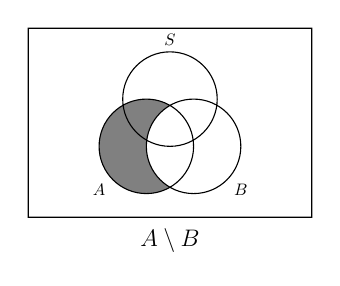
\begin{tikzpicture}[fill=gray, scale = .6, transform shape]
            %A \setminus B
            \scope
            \clip (-3,-2) rectangle (3,2)
                  (.5,-.5) circle (1);
            \fill (-.5,-.5) circle (1);
            \endscope
            % outline
            \draw (-.5,-.5) circle (1) (-1.5,-1.41) node [text=black] {$A$}
                  (0,.5) circle (1) (0,1.5)  node [text=black, above] {$S$}
                  (.5,-.5) circle (1) (1.5,-1.41) node [text=black] {$B$}
                  (-3,-2) rectangle (3,2)
                  (0, -2.5) node {{\Large $A \setminus B$}};
        \end{tikzpicture} &
        &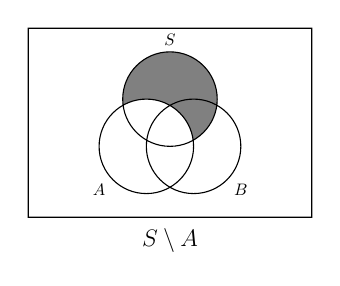
\begin{tikzpicture}[fill=gray, scale = .6, transform shape]
            %S \setminus A
            \scope
            \clip (-3,-2) rectangle (3,2)
                  (-.5,-.5) circle (1);
            \fill (0,.5) circle (1);
            \endscope
            % outline
            \draw (-.5,-.5) circle (1) (-1.5,-1.41) node [text=black] {$A$}
                  (0,.5) circle (1) (0,1.5)  node [text=black, above] {$S$}
                  (.5,-.5) circle (1) (1.5,-1.41) node [text=black] {$B$}
                  (-3,-2) rectangle (3,2)
                  (0, -2.5) node {{\Large $S \setminus A$}};
        \end{tikzpicture} &
        &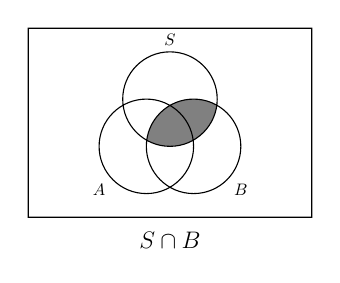
\begin{tikzpicture}[fill=gray, scale = .6, transform shape]
            %S \cap B
            \scope
            \clip (0,.5) circle (1);
            \fill (.5,-.5) circle (1);
            \endscope
            % outline
            \draw (-.5,-.5) circle (1) (-1.5,-1.41) node [text=black] {$A$}
                  (0,.5) circle (1) (0,1.5)  node [text=black, above] {$S$}
                  (.5,-.5) circle (1) (1.5,-1.41) node [text=black] {$B$}
                  (-3,-2) rectangle (3,2)
                  (0, -2.5) node {{\Large $S \cap B$}};
        \end{tikzpicture}
        \end{align*}
        \vspace{-\belowdisplayskip}
        \vspace{-\abovedisplayskip}
        \begin{align*}
        &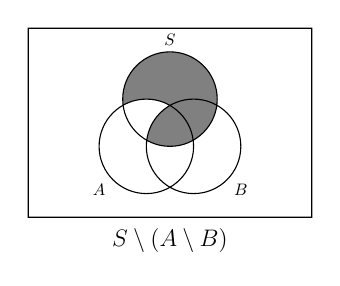
\begin{tikzpicture}[fill=gray, scale = .6, transform shape]
            %S \setminus (A \cap B)
            \scope
            \clip (-2.5,-2) rectangle (2.5,2)
                  (-.5,-.5) circle (1)
                  (.5,-.5) circle (1);
            \fill (0,.5) circle (1);
            \endscope
            %S \cap B
            \scope
            \clip (0,.5) circle (1);
            \fill (.5,-.5) circle (1);
            \endscope
            % outline
            \draw (-.5,-.5) circle (1) (-1.5,-1.41) node [text=black] {$A$}
                  (0,.5) circle (1) (0,1.5)  node [text=black, above] {$S$}
                  (.5,-.5) circle (1) (1.5,-1.41) node [text=black] {$B$}
                  (-3,-2) rectangle (3,2)
                  (0, -2.5) node {{\Large $S \setminus (A \setminus B)$}};
        \end{tikzpicture} &
        &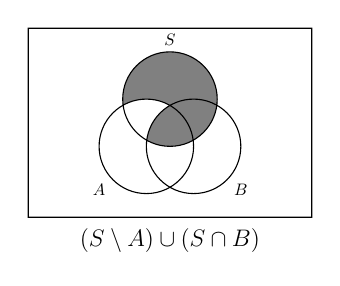
\begin{tikzpicture}[fill=gray, scale = .6, transform shape]
            %S \setminus (A \cap B)
            \scope
            \clip (-2.5,-2) rectangle (2.5,2)
                  (-.5,-.5) circle (1)
                  (.5,-.5) circle (1);
            \fill (0,.5) circle (1);
            \endscope
            %S \cap B
            \scope
            \clip (0,.5) circle (1);
            \fill (.5,-.5) circle (1);
            \endscope
            % outline
            \draw (-.5,-.5) circle (1) (-1.5,-1.41) node [text=black] {$A$}
                  (0,.5) circle (1) (0,1.5)  node [text=black, above] {$S$}
                  (.5,-.5) circle (1) (1.5,-1.41) node [text=black] {$B$}
                  (-3,-2) rectangle (3,2)
                  (0, -2.5) node {{\Large $(S \setminus A) \cup (S \cap B)$}};
        \end{tikzpicture}
        \end{align*}


\subsection*{Question 3}
    Let $A$ and $B$ be sets and let $x$ be any object. Prove that $x \notin A \setminus B$ iff $x \notin A$ or $x \in B$.

\subsection*{Solution}
    Using one of De Morgan's laws for propositional logic, we have 
    \begin{align*}
        & x \notin A \setminus B \\
        \text{iff } & \text{it is not the case that $x \in A \setminus B$} \\
        \text{iff } & \text{it is not the case that $x \in A$ and $x \notin B$} \\
        \text{iff } & \text{$x \notin A$ or $x \in B$}.
    \end{align*}

\subsection*{Question 4}
    Let $A$, $B$, $C$, and $D$ be sets. Suppose $B$ and $D$ are nonempty. Prove that if $A \times B = C \times D$, then $A = C$.

\subsection*{Solution}
    We are given $B \ne \emptyset$ and $D \ne \emptyset$. Suppose $A \times B = C \times D$. We wish to prove that $A = C$.
    \begin{enumerate} [label = \arabic*.]%Part 1 and part 2
        \item To prove $A \subseteq C$. Let $a \in A$. Since $B \ne \emptyset$, we pick $b_0 \in B$. Then $(a, b_0) \in A \times B$. Since $A \times B = C \times D$, we get $(a, b_0) \in C \times D$.  By definition of Cartesian product, we get $a \in C$ and $b_0 \in D$. Since $a \in C$, we have proved $A \subseteq C$.
        \item To prove $C \subseteq A$. Let $c \in C$. Since $D \ne \emptyset$, we pick $d_0 \in D$. Then $(c, d_0) \in C \times D$. Since $C \times D = A \times B$, we get $(c, d_0) \in A \times B$.  By definition of Cartesian product, we get $c \in A$ and $d_0 \in B$. Since $c \in A$, we have proved $C \subseteq A$.
    \end{enumerate}
    Since $A \subseteq C$ and $C \subseteq A$, we conclude that $A = C$.


\subsection*{Question 5 (Challenge)\footnotemark[1]}
    \fancyfootnotetext{1}{This question was taken from The Ohio State University.}
    
    Completing this problem, I feel, means you are adequately prepared for quiz/test questions on set theory. You may want to use the previous parts to solve the parts that appear after.
    Let $X$, $A$, $B$ be sets.
    \begin{enumerate}
        \item Prove that $X \setminus (B \setminus A)  = (X \setminus B) \cup (X \cap A).$
        \item Deduce that $X \setminus (X \setminus A) = X \cap A$.
        \item Prove that if $A \subseteq B$, then $X \setminus B \subseteq X \setminus A$.
        \item Prove that $A \subseteq X$ if and only if $A = X \setminus (X \setminus A)$.
        \item Suppose that $A \subseteq X$. Prove that if $X \setminus B \subseteq X \setminus A$, then $A \subseteq B$.
    \end{enumerate}

\subsection*{Solution}
    \begin{enumerate}
        \item \hfill
        $\begin{aligned}[t]
            X \setminus (B \setminus A) &= X \cap (B \cap A^c)^c = X \cap (B^c \cup A) \\
            &= (X \cap B^c) \cup (X \cap A) = (X \setminus B) \cup (X \cap A).
        \end{aligned}$ \hfill\null
        \item From part (a), we have $X \setminus (X \setminus A) = (X \setminus X) \cup (X \cap A) = X \cap A$. 
        \item Suppose $A \subseteq B$. Now using the law of contraposition, we have $B^c \subseteq A^c$. Then $X \cap B^c \subseteq X \cap A^c$. Hence by definition, $X \setminus B \subseteq X \setminus A$.
        \item We have $A \subseteq X$ iff $A = A \cap X$. From part (b), we know $A \cap X = X \setminus (X \setminus A).$ Hence $A \subseteq X$ iff $A = X \setminus (X \setminus A)$.
        \item We are given $A \subseteq X$. Suppose $X \setminus B \subseteq X \setminus A$. Then it follows from part (c) that $X \setminus (X \setminus A) \subseteq X \setminus (X \setminus B)$. Since $A \subseteq X$, from part (d) we have $A = X \setminus (X \setminus A)$. Now $X \setminus (X \setminus A) \subseteq X \setminus (X \setminus B)$ and $A = X \setminus (X \setminus A)$, so $A \subseteq X \setminus (X \setminus B)$. From part (b), we know $X \setminus (X \setminus B) = B \cap X$. Since $B \cap X \subseteq B$, it follows that $X \setminus (X \setminus B) \subseteq B$. Now $A \subseteq X \setminus (X \setminus B)$ and $X \setminus (X \setminus B) \subseteq B$, so $A \subseteq B$.
    \end{enumerate}

\subsection*{Question 6}
    Find and prove the size of any power set $\mathcal{P}(A)$, where $A$ is an arbitrary set such that $|A| = n$. 
    
    \vspace{1.5mm}{\small \textit{Hint:} The proof follows inductively. We have not covered induction yet, so if you are not familiar, it will suffice simply to make observations and guess.}

\subsection*{Solution}
    We claim by observation that the size of any power set $A$ is $2^{n}$, where $n$ is the number of elements of $A$, and shall prove so using induction.
    Let $P(n)$ be the sentence $$|\mathcal{P}(A)| = 2^{n}.$$
    \textsc{Base Case}: $P(0)$ is true, since the only subset of the empty set is the empty set itself, so $|\mathcal{P}(A)| = 1 = 2^{0}$. \\
    \textsc{Inductive Step}: Now let $n \in \mathbb{N}$ such that $P(A)$ is true. Let $B$ be a set with $n + 1$ elements, such as $B = X \cup \{b\}$. There are two types of subsets of $B$: those that include $b$ and those that exclude $b$. The latter are exactly the subsets of $A$, while the former are of the form $\mathcal{P}(A) \cup \{b\}$. By the inductive hypothesis, both have $2^{n}$ elements. Therefore, the total number of subsets of $B$ is $2^{n} + 2^{n} = 2^{n + 1}$. Hence $P(n + 1)$ is true as well. \\
    \textsc{Conclusion}: Therefore by induction, for all $n \in \mathbb{N}$, $P(n)$ is true.


\end{document}